\documentclass[11pt,a4paper]{article}

\usepackage[margin=1in]{geometry}
\usepackage{amsmath,amssymb,booktabs,array,graphicx,hyperref,microtype}
\usepackage{enumitem}
\usepackage{float}
\usepackage{xcolor}
\hypersetup{hidelinks}
\setlist{itemsep=2pt,topsep=4pt}

\title{Reliability-Screened Routing Under Predictable and Stochastic Travel Variation\\
\large Matched Comparisons of Conservative Planning and Statistical Screening}
\author{Suhan Ali\\[2pt]\small Independent researcher, Lahore, Pakistan\\
\small \href{mailto:syedsuhanali9@gmail.com}{syedsuhanali9@gmail.com}\quad
ORCID: \href{https://orcid.org/0009-0004-5079-7684}{0009-0004-5079-7684}}
\date{September 2026}
\newcommand{\ProcConsRange}{8.3--21.4}
\newcommand{\ConservativeSelected}{25}
\newcommand{\ConservativeRetained}{25}
\newcommand{\CappedSelected}{42}
\newcommand{\CappedRetained}{40}
\newcommand{\OriginalRetained}{30}
\newcommand{\OriginalProbability}{78.9}
\newcommand{\ConservativeProbability}{78.6}
\newcommand{\CappedProbability}{86.6}
\newcommand{\ClockFound}{49}
\newcommand{\CappedGainInterval}{7.7 [3.5, 12.5]}
\newcommand{\CappedDistanceCost}{2.5}
\newcommand{\CappedFleetCost}{0.43}
\newcommand{\OriginalSelected}{32}
\newcommand{\FailureCount}{21}
\newcommand{\CertifiedFailures}{17}
\newcommand{\SweepLowIndep}{-3.1}
\newcommand{\SweepHighIndep}{30.5}
\newcommand{\CappedLargeRange}{97.5--97.6}
\newcommand{\CappedLargeSelected}{18/18}
\newcommand{\CappedLargeRetained}{16/18}
\newcommand{\OriginalSelectedMean}{97.3}
\newcommand{\OriginalFallbackMean}{50.9}
\newcommand{\CappedSelectedMean}{97.4}
\newcommand{\CappedFallbackMean}{45.2}
\newcommand{\CappedFallbackCount}{11}
\newcommand{\BudgetDiagCases}{8}
\newcommand{\BudgetDiagSearchLimits}{4}
\newcommand{\BudgetDiagUnresolved}{4}
\newcommand{\CappedFleetLarge}{1.88}

\begin{document}
\maketitle

\begin{abstract}
Delivery routes planned on nominal travel times can satisfy every time window
on paper yet fail under predictable congestion and random delay. This paper
audits a two-layer procedure for the capacitated vehicle-routing problem with
time windows. Replaceable OR-Tools generators propose plans, internal window
contraction supplies candidate buffers without changing customer promises,
and a plan is admitted only when a one-sided 95\% Wilson lower bound on the
probability that at least 95\% of customers are served on time reaches 0.95.
Selected plans are then assessed once on untouched scenarios. On 53 seeded
synthetic instances with 20--200 customers, three findings emerge. First, on
the 46 instances where both exist, the screened procedure exceeds uniformly
conservative travel-time padding by \ProcConsRange{} percentage points, and for
independent disturbances the gap rises from $\SweepLowIndep$ to
\SweepHighIndep{} points as the log-error scale grows from 0.10 to 0.30.
Second, among the \FailureCount{} instances without an admitted plan,
\CertifiedFailures{} encounter a certified reachability obstruction at one or
more tested contraction levels. Third, capping
each customer's contraction at its direct-reachability limit raises admission
from \OriginalSelected{} to \CappedSelected{} instances and pooled service
probability from \OriginalProbability\% to \CappedProbability\%, averaging
\CappedLargeRange\% at 100 and 200 customers, at \CappedDistanceCost\% more
distance and \CappedFleetCost{} more vehicles per instance. Pooled performance
remains below the 95\% target. These findings are exploratory, because the
same instances informed the design; a prespecified confirmatory protocol for
fresh instances accompanies the archive.
\end{abstract}

\section{Introduction}

The vehicle-routing problem with time windows (VRPTW) asks a fleet to serve
geographically distributed customers subject to capacity and scheduling
constraints \cite{solomon1987,toth2014}. In practice, a route that is feasible
under one planning-time matrix may miss promised windows when congestion varies
or small delays propagate downstream. Minimising nominal distance alone does
not price that fragility.

This paper asks four questions:
\begin{enumerate}
  \item Does the complete screened procedure improve on uniformly
        conservative planning when both are compared on identical instances?
  \item Does any remaining reliability gain arise from route structure or
        simply from using more vehicles?
  \item How do generator choice, clock-profile information and individual
        contraction caps change admission success and out-of-sample service?
  \item How much distance, driver duration, and fleet use are exchanged for the
        resulting reliability?
\end{enumerate}

The proposed architecture separates \emph{candidate generation} from
\emph{stochastic validation}. This distinction is central. The optimizer is a
nominal VRPTW solver and is not presented as an exact solver for a
time-dependent stochastic program. Candidate routes are stress-tested after
solving, first on a screening bank and then once on an untouched validation
bank. The principal reliability event permits a small daily proportion of late
deliveries, avoiding the mechanical collapse of an all-customers-on-time
probability as instance size grows.

The contribution is integrative rather than component-wise. Time-dependent
speed profiles, multi-criteria routing, chance constraints, Monte Carlo
evaluation, and Wilson intervals are established ideas. The contribution is a
reproducible pipeline that keeps their roles statistically and computationally
separate, together with ablations of uniform travel-time padding, clock-profile
information, fleet resources, contracted candidates and screening. The
screened family and the statistical selection rule act together; a contrast
against one uncontracted plan does not identify the selection rule alone.

\section{Related work}

Solomon's benchmark study established the standard VRPTW experimental setting
\cite{solomon1987}; Toth and Vigo provide a broad treatment of vehicle-routing
models and algorithms \cite{toth2014}. Time-dependent routing requires care
because a naive multiplier applied at departure can violate first-in-first-out
(FIFO). Ichoua, Gendreau, and Potvin introduced the integrated speed-profile
construction used here \cite{ichoua2003}; Ghiani and Guerriero later analysed
its representational properties \cite{ghiani2014}.

Stochastic VRPTW research has treated uncertain travel and service times using
chance constraints, recourse, approximate route-feasibility tests, and
data-driven formulations \cite{li2010,errico2018,bomboi2022,serrano2026}.
Ehmke, Campbell, and Urban embed per-customer service levels in a routing
method \cite{ehmke2015}; Ta\c{s} et al. jointly model time dependence,
stochastic travel, service costs, and soft windows \cite{tas2014}; and Bomboi,
Buchheim, and Pruente develop route-feasibility checks for correlated and
time-dependent travel times \cite{bomboi2022}. Vareias, Repoussis, and
Tarantilis optimize self-imposed time windows under stochastic travel times
\cite{vareias2019}, which is the closest conceptual analogue to the internal
window contraction used here.

The present method differs in where the statistical claim is made. It does not
embed a stochastic feasibility approximation inside a specialist route-search
algorithm. Instead, it accepts routes from a replaceable nominal solver,
searches an internal-buffer family on one scenario bank, and audits the chosen
plan once on a held-out bank. Its daily service event constrains the proportion
of customers served on time rather than imposing the same marginal chance
constraint at every customer. This solver-agnostic separation is narrower than
a new stochastic optimizer, but makes selection failure and out-of-sample
reliability directly observable. Monte Carlo approximations to chance
constraints require separate assessment of candidate feasibility
\cite{ahmed2008}; the Wilson bound is used because normal intervals behave
poorly near probabilities close to one \cite{wilson1927,brown2001}.

The implementation uses Google OR-Tools as a nominal candidate generator
\cite{ortools}. It is a practical local-search framework, not an exact method.
PyVRP provides a substantially stronger hybrid genetic search benchmark for
canonical VRPTW variants \cite{wouda2024}; comparison with such solvers is
necessary before interpreting absolute route quality as state of the art.

\section{Problem definition}

Let $N=\{0,1,\ldots,n\}$ be the nodes, with depot 0 and customers
$C=N\setminus\{0\}$. Let $V$ be a homogeneous fleet. Customer $i$ has demand
$\delta_i$, deterministic service time $s_i$, and offered service-start window
$[l_i,u_i]$. Vehicle capacity is $Q$, and the maximum shift duration is
$H^{\max}$. The nominal distance and planning time on arc $(i,j)$ are $d_{ij}$
and $\bar t_{ij}$.

The planning variables are $x_{ijv}\in\{0,1\}$ for arc use,
$z_{iv}\in\{0,1\}$ for customer assignment, $y_v\in\{0,1\}$ for vehicle use,
service-start time $a_{iv}$, depot departure $d_v$, depot return $r_v$, and
slack deficit $G_{iv}\geq0$. Assignment variables explicitly activate the
customer--vehicle copies:
\begin{align}
 \sum_{v\in V} z_{iv} &= 1 && i\in C, \\
 \sum_{j\in N\setminus\{i\}}x_{ijv}
   =\sum_{j\in N\setminus\{i\}}x_{jiv} &= z_{iv}
      && i\in C,\ v\in V, \\
 \sum_{j\in C}x_{0jv}=\sum_{i\in C}x_{i0v} &= y_v
      && v\in V.                                            \label{eq:flow}
\end{align}
For delivery-only demand, route capacity can be stated without cumulative-load
variables:
\begin{equation}
 \sum_{i\in C}\delta_i z_{iv}\leq Qy_v \qquad v\in V.       \label{eq:capacity}
\end{equation}
The time-propagation constraints exclude customer-only subtours: summing them
around any directed customer cycle would imply
$0\geq\sum_i(s_i+\bar t_{ij})>0$. Positive demands are not needed for that
argument. Time windows are activated rather than imposed on unassigned copies:
\begin{equation}
 l_i z_{iv}\leq a_{iv}\leq u_i z_{iv}
 \qquad i\in C,\ v\in V.                                   \label{eq:activate}
\end{equation}
Using separate departure and return variables avoids representing two depot
visits with one time variable. With a valid global deactivation constant
$M\geq H^{\max}+\max_i s_i+\max_{ij}\bar t_{ij}$,
\begin{align}
 a_{jv} &\geq d_v+\bar t_{0j}-M(1-x_{0jv}), \\
 a_{jv} &\geq a_{iv}+s_i+\bar t_{ij}-M(1-x_{ijv}), \\
 r_v &\geq a_{iv}+s_i+\bar t_{i0}-M(1-x_{i0v}).              \label{eq:time}
\end{align}
The bounds $0\leq d_v,r_v\leq H^{\max}y_v$ deactivate unused vehicles, and
$r_v-d_v\leq H^{\max}y_v$. The implementation uses OR-Tools Routing
dimensions rather than explicitly instantiating \eqref{eq:time}; consequently,
no big-$M$ relaxation or big-$M$ diagnostic is claimed for the code.

For target slack $s^*$,
\begin{align}
 G_{iv} &\geq a_{iv}-(u_i-s^*)z_{iv}, \\
 G_{iv} &\geq 0.                                            \label{eq:slack}
\end{align}
This makes $G_{iv}=\max\{0,s^*-(u_i-a_{iv})\}$ when $z_{iv}=1$ and zero when
the customer is not assigned to vehicle $v$.

\section{Candidate objectives and scaling}\label{sec:objective-scaling}

The four raw criteria are
\begin{align}
 F_1 &= c_f\sum_{v\in V}\sum_{i,j\in N}d_{ij}x_{ijv},
 &F_2 &= \sum_{v\in V}\sum_{i\in C}G_{iv},\\
 F_3 &= \sum_{v\in V}(r_v-d_v),
 &F_4 &= \sum_{v\in V}y_v.                                 \label{eq:criteria}
\end{align}
Thus $F_3$ includes driving, service, and waiting while permitting each vehicle
to depart when useful. This removes the fixed-departure artifact that charged a
vehicle for depot waiting before its first feasible service.

Single-criterion heuristic solves provide empirical reference values. For each
criterion $k$, let $L_k$ and $U_k$ be the smallest and largest values observed
across these anchor solutions. These values are \emph{scaling ranges}, not
utopia and nadir points, and they need not contain the Pareto frontier. No value
is clipped. The normalized score is
\begin{equation}
 Z(x)=\sum_{k=1}^{4}w_k\frac{F_k(x)-L_k}{\max\{U_k-L_k,1\}}. \label{eq:objective}
\end{equation}
The unit fallback prevents division by zero when the anchor archive shows no
variation in a discrete criterion. The baseline weights
$w=(0.5693,0.2643,0.1055,0.0609)$ are the principal-eigenvector weights of a
single AHP pairwise-comparison matrix with consistency ratio 0.0254
\cite{saaty1980}; the matrix and calculation appear in
Appendix~\ref{sec:ahp-matrix} and in \texttt{code/ahp\_weights.py}. The matrix
was specified for an earlier criteria set in which the third criterion was
total distance, and its third row and column were not re-elicited when that
criterion became driver duration. The weights therefore express one
illustrative preference ordering, fixed before any experiment reported here;
they were not elicited from a fleet operator, and sensitivity to them is not
evaluated.

OR-Tools implements the distance term as an arc cost, driver duration as a
per-vehicle Time-dimension span cost, slack deficit as customer soft upper
bounds, and fleet use as a fixed vehicle cost. Integer coefficients are scaled
once at the criterion level. The primary planning matrix is nominal and fixed;
the original candidate generator does not use clock-dependent costs. The
\emph{conservative-speed} baseline replaces 40 km/h by 33.3 km/h throughout
the planning matrix. It pads all trips by 20\%, including off-peak trips; it
does not isolate knowledge of the peak's timing.

\subsection{Clock-aware approximation and deterministic guarantee}

A separate distance heuristic freezes each origin's estimated departure from
the preceding schedule, integrates \eqref{eq:fifo} at that time to construct an
outgoing travel-time row, and re-solves. Two passes receive 2.5 seconds each.
The first reference is the retained nominal plan, whose separate solve cost
has already been incurred. Customer departures are
estimated service start plus service time; for depot arcs, the estimate is the
preceding departure for the first customer of each route, or the mean of used
depot departures for other customers. Each resulting sequence is rescheduled
with the exact deterministic FIFO profile. Binary search finds its latest
feasible whole-minute depot departure; routes failing at departure zero are
rejected. The shortest deterministically feasible output is retained, with
duration breaking ties. This is an approximation with explicit failure
reporting, not a departure-dependent callback or an exact TDVRPTW optimizer.

For a feasible conservative-speed plan, the evaluation speed at $\sigma=0$
never falls below the planning speed during the planned shift. Starting from
the same depot departure, FIFO and induction along each route imply that
evaluated service starts and return occur no later than their planned times.
Thus deterministic 100\% on-time service is guaranteed by construction.
The clock-aware approximation's deterministic feasibility is likewise checked
before acceptance. These properties are not experimental reliability gains.

\section{Time-dependent stochastic evaluation}

\subsection{FIFO travel times}

Partition the day into periods $[T_k,T_{k+1})$ with strictly positive speeds
$\nu_k$. The deterministic time-dependent travel time $t_{ij}(\tau)$ is the
smallest $\Delta\geq0$ satisfying
\begin{equation}
 \int_{\tau}^{\tau+\Delta}\nu(u)\,du=d_{ij},
 \qquad \nu(u)=\nu_k\text{ for }u\in[T_k,T_{k+1}).           \label{eq:fifo}
\end{equation}
Because distance accumulated by time is strictly increasing, the arrival map
$\tau\mapsto\tau+t_{ij}(\tau)$ is nondecreasing and FIFO holds.

\subsection{Correlated disturbances}

For scenario $\omega$, arc travel is
\begin{equation}
 T_{ij}(\tau,\omega)=t_{ij}(\tau)\Omega_{ij}(\omega),
\end{equation}
where
\begin{align}
 \Omega_{ij}(\omega)&=\exp\{\varepsilon_{ij}(\omega)\},\\
 \varepsilon_{ij}(\omega)&=\sigma\left(
 \sqrt{\rho}\,\xi_0(\omega)+\sqrt{1-\rho}\,\xi_{ij}(\omega)\right).
                                                               \label{eq:noise}
\end{align}
Here $\rho$ is the correlation between latent Gaussian log-errors. It is not
the Pearson correlation between multipliers, which equals
\begin{equation}
 \operatorname{Corr}(\Omega_i,\Omega_j)
 =\frac{\exp(\sigma^2\rho)-1}{\exp(\sigma^2)-1}.
\end{equation}
The multiplier has median 1 and mean $\exp(\sigma^2/2)$, so the deterministic
profile represents a median rather than a mean travel condition.

Scenario banks are generated independently of route iteration order. A common
factor is drawn once per scenario, while each directed arc receives a
deterministic pseudorandom stream keyed by the bank seed and arc endpoints.
Plans evaluated on the same bank therefore experience identical disturbances
on shared arcs.

\section{Screening and independent validation}

For a fixed plan $R$ and scenario $\omega$, let
\begin{equation}
 q(R,\omega)=\frac{1}{|C|}\sum_{i\in C}
 \mathbf{1}\{a_i(R,\omega)\leq u_i\}
\end{equation}
be the on-time customer proportion. The primary service event is
\begin{equation}
 J_{\kappa}(R,\omega)=\mathbf{1}\{q(R,\omega)\geq\kappa\},
 \qquad \kappa=0.95,                                        \label{eq:event}
\end{equation}
and the target is
\begin{equation}
 \Pr[J_{\kappa}(R,\omega)=1]\geq\alpha,
 \qquad \alpha=0.95.                                       \label{eq:chance}
\end{equation}
The stricter zero-lateness fleet-day probability is still reported, but is not
the sole admission condition because it declines mechanically as the number of
customers increases.

For $N$ scenarios and empirical success $\hat p$, the one-sided Wilson lower
bound at confidence $1-\eta$ is
\begin{equation}
 L(\hat p)=
 \frac{\hat p+z^2/(2N)-z\sqrt{\hat p(1-\hat p)/N+z^2/(4N^2)}}
 {1+z^2/N},\qquad z=z_{1-\eta}.                             \label{eq:wilson}
\end{equation}

Candidate generation contracts only the internal planning deadline:
$[l_i,\max\{l_i,u_i-\beta\}]$. The offered window $[l_i,u_i]$ is unchanged, and every
scenario is scored against the original $u_i$. Candidate values of $\beta$ are
generated with the slack-aware objective and assessed on a screening bank. The
anchor ranges are computed once from the uncontracted ($\beta=0$) instance and
held fixed over the buffer search. Among candidates whose screening lower bound
reaches $\alpha$, the one with the smallest normalized planned score
\eqref{eq:objective} is selected. In simulation, every vehicle departs at its
planned $d_v$; there is no scenario-dependent departure recourse. The selected
plan is evaluated once on a larger, untouched validation bank. This separation
prevents adaptive candidate search from selecting on the evidence used for
final reporting.

For procedure-level reporting, a prespecified fallback makes the output defined
on every instance. If no candidate passes screening, the uncontracted
slack-aware plan ($\beta=0$) is returned. Validation never changes this choice:
it estimates performance rather than retrospectively selecting a different
plan. Selected-only results are shown only when labelled as such; the primary
procedure comparison includes all instances.

\subsection{Generator replacement and reachability-capped contraction}

Screened conservative-speed uses the same buffer grid, admission bank and
Wilson threshold, but generates distance-minimizing plans with the padded
matrix. Among passing plans it chooses the shortest distance, breaking ties by
planned duration and then buffer. Its fallback is the uncontracted
conservative plan; if that plan was not found, the retained uncontracted
slack-aware plan is used. This makes the replacement procedure defined on all
53 instances while preserving the base generator's 46/53 found-plan count.

Let $e_i=\max\{l_i,\bar t_{0i}\}$ be earliest direct service under the nominal
matrix. The capped weighted variant uses the internal upper bound
\begin{equation}
 u_i^{\rm cap}(\beta)=\min\{u_i,\max\{l_i,u_i-\beta,e_i\}\}.
\end{equation}
This prevents an initially reachable customer from becoming unreachable by a
direct trip solely because of contraction. It does not imply joint routing
feasibility or the admission target. Identical contracted models reuse their
archived candidates; only changed models are re-solved. Selection still uses
the fixed original scaling ranges and weighted score, with the same fallback.

For diagnosis, a shortest-path relaxation uses arc cost
$\bar t_{ij}+s_i$ (with $s_0=0$), allowing intermediate customers without
capacity or window restrictions. Its depot-to-$i$ distance is a valid lower
bound even if rounded distances violate a triangle inequality. A contracted
deadline below this bound certifies infeasibility. Without a certificate, a
missing solver output is labelled \emph{no feasible plan found}; neither a
time limit nor passing the reachability test proves feasibility. Solver
status certificates were not retained in the archived runs and are not
inferred retrospectively.

\section{Experimental design}

Synthetic instances place a central depot and uniformly distributed customers
on a $100\times100$ grid. Demand is uniform on 10--49 units, service time is
10 minutes, window width is uniform on 90--149 minutes, capacity is 1000, and
the shift limit is 600 minutes. Time zero is 06:00 local time, so simulated
clock time is obtained by adding 360 minutes to each relative schedule time.
The retained design uses the seeded sizes in Table~\ref{tab:design}; all model
and simulation constants are disclosed in Table~\ref{tab:parameters}.

\begin{table}[ht]
\centering
\caption{Seeded synthetic experimental design.}
\label{tab:design}
\begin{tabular}{rrrr}
\toprule
Customers & Vehicles available & Instances & Seeds\\
\midrule
20  & 6  & 20 & 7200--7219\\
50  & 14 & 15 & 7500--7514\\
100 & 26 & 10 & 8000--8009\\
200 & 40 & 8  & 9000--9007\\
\bottomrule
\end{tabular}
\end{table}

\begin{table}[ht]
\centering
\small
\caption{Planning, disturbance, and statistical parameters.}
\label{tab:parameters}
\begin{tabular}{p{0.42\textwidth}p{0.46\textwidth}}
\toprule
Parameter & Retained value \\
\midrule
Nominal/free-flow speed $\bar v$ & 40 km/h \\
Shift and clock origin & 600 min, beginning 06:00 local time \\
Capacity; service time; target slack $s^*$ & 1000; 10 min; 15 min \\
Distance cost $c_f$ & 15 cost units/km \\
AHP weights $(w_1,w_2,w_3,w_4)$ & $(0.5693,0.2643,0.1055,0.0609)$ \\
Integer objective scale & 100,000 \\
Planned-shift speed divisors &
$0.9$ (06:00--07:00), $1.2$ (07:00--09:00), and $1.0$
(09:00--16:00); speed is $\bar v$ divided by the divisor \\
Outside-shift continuation & 1.0 to 17:00, 1.3 (17:00--19:00), 0.9 thereafter;
used if a stochastic route overruns the shift \\
Log-error scale $\sigma$; latent correlation $\rho$ & 0.20; 0.50 \\
Exploratory disturbance grid & $\sigma\in\{0.10,0.20,0.30\}$;
$\rho\in\{0,0.5,0.9\}$ \\
Service fraction $\kappa$; target $\alpha$ & 0.95; 0.95 \\
Wilson tail probability $\eta$ & 0.05 (one-sided 95\% lower bound) \\
Screening; validation; sensitivity scenarios & 1000; 5000; 1000 per cell \\
Buffer grid & $\beta\in\{0,5,\ldots,60\}$ min \\
\bottomrule
\end{tabular}
\end{table}

Eight configurations are compared:
\begin{enumerate}
  \item \textbf{Nominal distance}: fixed 40 km/h planning matrix and a
        distance-minimizing objective.
  \item \textbf{Conservative-speed distance}: distance minimization with a
        uniform 33.3 km/h planning matrix.
  \item \textbf{Slack-aware}: objective \eqref{eq:objective} with $\beta=0$,
        isolating the objective from screening.
  \item \textbf{Fleet-matched distance}: distance minimization forced to use
        exactly the fleet count of the slack-aware plan and initialized from
        its feasible routes.
  \item \textbf{Original procedure}: the complete weighted internal-buffer search, with
        selection on 1000 screening scenarios, the prespecified $\beta=0$
        fallback, and assessment on 5000 fresh scenarios.
  \item \textbf{Screened conservative}: conservative-speed distance candidates
        with the same admission test and the fallback defined above.
  \item \textbf{Capped procedure}: the original weighted procedure with
        customer-specific reachability caps.
  \item \textbf{Clock approximation}: two departure-estimate matrix updates
        and exact deterministic route rescheduling.
\end{enumerate}

The nominal shift ends at 16:00. The full-day speed profile remains defined
beyond that time because lognormal delays are unbounded and a stochastic
route can overrun. Evening periods are outside the planned shift, not removed
from the evaluator. Fleet-matched distance is initialized from the slack-aware
routes; this can in principle transfer their structure, so it is disclosed as
part of the comparator, not treated as an independent random initialization.

The screening grid is $\beta\in\{0,5,\ldots,60\}$ minutes. The four
single-criterion anchor solves use two seconds each to stabilize the scaling
ranges; reported candidate configurations use a five-second OR-Tools search
budget for each nominal solve. If a candidate solve
returns no feasible plan, the same five-second call is attempted at most twice
more; the first feasible result is retained rather than taking the best of
multiple feasible runs. Reachability-certified new models need no solver
attempt. The clock approximation instead divides a total five-second budget
between its two solves. Six experiment workers ran in parallel; elapsed time
and software metadata are retained. All configurations use the same fresh
validation bank within an instance. The reported reliability outcomes
are service-event probability, zero-lateness fleet-day probability, mean
on-time fraction, expected number late, mean and 95th-percentile total
lateness, and mean route success. Operational outcomes are distance, driver
duration, and fleet use. Simulated duration is additionally reported under the
common evaluation model, to distinguish actual route time from each generator's
planned $F_3$. Differences are paired by instance. Confidence
intervals across instances are distinguished from binomial Monte Carlo
intervals within an instance. Across-instance intervals use a paired
nonparametric bootstrap with 20,000 resamples and a fixed analysis seed. Claims
of distance equivalence require a
pre-specified equivalence margin; failure to reject a difference is not treated
as proof of equality.

\section{Results}

\subsection{Complete procedures on matched instances}

Table~\ref{tab:matched} puts every original configuration on the same conservative-feasible subset. The paired contrasts are computed from individual instance differences. Their intervals therefore quantify the comparison directly; they are not obtained by subtracting endpoints of separate confidence intervals.

\begin{table}[htbp]
\centering
\scriptsize
\caption{Validated service-event probability (\%) on the same 46 instances: every entry in a row has the displayed denominator. Entries are mean [95\% instance-bootstrap interval]. N, C, S, F and P denote nominal, conservative-speed, slack-aware, fleet-matched and original procedure, respectively.}
\label{tab:matched}
\begin{tabular}{rrlllll}
\toprule
$n$ & $k$ & N & C & S & F & P\\
\midrule
20 & 18 & 21.5 [18.8, 24.4] & 64.2 [61.1, 67.4] & 53.3 [47.6, 59.4] & 21.7 [18.9, 24.8] & 85.7 [74.4, 95.0]\\
50 & 13 & 17.7 [16.1, 19.6] & 59.0 [54.6, 63.1] & 45.8 [43.1, 48.4] & 16.9 [14.8, 18.9] & 76.8 [62.3, 89.7]\\
100 & 8 & 25.4 [23.5, 27.1] & 71.6 [69.1, 74.0] & 55.3 [51.5, 59.3] & 26.2 [23.6, 29.0] & 87.6 [74.2, 97.5]\\
200 & 7 & 26.7 [24.9, 28.8] & 74.6 [72.2, 77.0] & 61.7 [58.3, 66.8] & 27.7 [25.5, 30.6] & 82.9 [69.3, 94.3]\\
\bottomrule
\end{tabular}
\end{table}


\begin{table}[htbp]
\centering
\small
\caption{Paired probability differences (percentage points) on exactly the same subsets as Table~\ref{tab:matched}. SC denotes screened conservative-speed with its prespecified fallback.}
\label{tab:paired}
\begin{tabular}{rlll}
\toprule
$n$ & S minus C & P minus C & SC minus C\\
\midrule
20 & $-$11.0 [$-$16.1, $-$6.0] & 21.4 [9.6, 31.3] & 28.2 [21.4, 34.3]\\
50 & $-$13.1 [$-$17.4, $-$8.9] & 17.9 [2.8, 32.0] & 11.8 [2.7, 22.2]\\
100 & $-$16.2 [$-$20.6, $-$11.7] & 16.0 [4.8, 24.8] & 11.2 [2.8, 19.4]\\
200 & $-$12.9 [$-$18.5, $-$5.7] & 8.3 [$-$5.1, 20.0] & 5.7 [0.0, 12.9]\\
\bottomrule
\end{tabular}
\end{table}


In the paired contrasts of Table~\ref{tab:paired}, the complete original procedure improves on conservative-speed planning by 8.3--21.4 percentage points across sizes. The unscreened slack-aware objective does not show this advantage. At $n=200$ the interval includes zero, so the positive mean at that size is not conclusive.

\subsection{Resources on the common subset}

\begin{table}[htbp]
\centering
\scriptsize
\caption{Paired original-procedure changes relative to conservative speed on the common subset. Distance and duration are mean percentage changes; fleet is an absolute difference. Scheduled duration is each planner's own $F_3$. Simulated duration uses the same realized traffic model and planned departures for both configurations.}
\label{tab:cost}
\begin{tabular}{rllll}
\toprule
$n$ & Distance & Scheduled time & Simulated time & Fleet\\
\midrule
20 & 4.9 [2.4, 7.3] & 0.3 [$-$3.8, 4.8] & 8.5 [4.4, 12.9] & 0.22 [0.00, 0.44]\\
50 & 2.3 [$-$0.6, 5.2] & $-$7.5 [$-$12.2, $-$2.7] & $-$2.0 [$-$7.0, 2.8] & $-$0.46 [$-$1.00, 0.00]\\
100 & 2.0 [$-$1.3, 5.1] & $-$3.0 [$-$9.4, 2.5] & 2.2 [$-$4.3, 7.6] & 0.12 [$-$0.38, 0.62]\\
200 & 2.4 [$-$1.4, 5.7] & $-$7.7 [$-$15.2, $-$1.0] & $-$2.8 [$-$10.6, 4.1] & $-$0.71 [$-$2.57, 1.00]\\
\bottomrule
\end{tabular}
\end{table}


Scheduled driver duration is not identical to realized labour time: the conservative planner budgets padded arc times, while the evaluator may traverse those arcs faster. Table~\ref{tab:cost} therefore includes both measures. Absolute distance premiums also carry solver-quality uncertainty: the five-second deterministic OR-Tools benchmark remains about 11\% longer than HGS at $n=200$.

The matched data do not support uniform resource dominance: at $n=20$ the original procedure has slightly greater scheduled time and more vehicles; at $n=100$ it also uses slightly more vehicles. The simulated-time interval excludes zero only for the increase at $n=20$. The service gain is therefore a trade-off against some operating resources.

\subsection{Screening a replaceable generator and capping contractions}

\begin{table}[htbp]
\centering
\small
\caption{All-instance procedure outcomes. Selected counts admission-bank lower bounds reaching 0.95; retained counts those selections whose fresh validation lower bound also reaches 0.95. Probability includes every fallback, as well as selected plans.}
\label{tab:screen}
\begin{tabular}{rllll}
\toprule
$n$ & Procedure & Selected / instances & Retained / selected & Probability (\%)\\
\midrule
20 & Original procedure & 14/20 & 14/14 & 81.6 [70.2, 91.9]\\
20 & Screened conservative & 15/20 & 15/15 & 87.7 [79.0, 94.7]\\
20 & Capped procedure & 14/20 & 14/14 & 81.6 [70.3, 92.0]\\
50 & Original procedure & 8/15 & 8/8 & 72.7 [59.2, 86.4]\\
50 & Screened conservative & 4/15 & 4/4 & 67.5 [58.2, 77.3]\\
50 & Capped procedure & 10/15 & 10/10 & 80.1 [66.9, 90.8]\\
100 & Original procedure & 6/10 & 5/6 & 81.3 [68.8, 93.3]\\
100 & Screened conservative & 4/10 & 4/4 & 77.5 [67.2, 88.2]\\
100 & Capped procedure & 10/10 & 9/10 & 97.5 [96.7, 98.2]\\
200 & Original procedure & 4/8 & 3/4 & 80.6 [68.7, 92.3]\\
200 & Screened conservative & 2/8 & 2/2 & 78.3 [71.0, 86.5]\\
200 & Capped procedure & 8/8 & 7/8 & 97.6 [96.9, 98.2]\\
\bottomrule
\end{tabular}
\end{table}


In Table~\ref{tab:screen}, the screened conservative generator selects on 25/53 instances; 25 selections retain the target lower bound. Its all-instance paired difference from the original procedure is $-$0.3 [$-$5.5, 5.0] points. The capped variant selects on 42/53, with 40 retained; its corresponding difference is 7.7 [3.5, 12.5] points. Capping removes only an individual reachability obstruction; capacity, sequencing and finite-search limitations remain.

\begin{table}[htbp]
\centering
\scriptsize
\caption{Operational price of the capped variant relative to the original procedure on all 53 instances. Percentage changes are paired per instance; fleet changes are absolute. Capping can permit different route and resource choices, so its reliability gain is not attributed to schedule structure alone.}
\label{tab:cap-cost}
\begin{tabular}{rllll}
\toprule
$n$ & Distance & Scheduled time & Simulated time & Fleet\\
\midrule
20 & 0.0 [0.0, 0.0] & 0.0 [0.0, 0.0] & 0.0 [0.0, 0.0] & 0.00 [0.00, 0.00]\\
50 & 2.2 [0.0, 5.4] & 4.6 [0.0, 11.4] & 4.5 [0.0, 11.3] & 0.33 [0.00, 0.87]\\
100 & 4.9 [1.1, 8.9] & 6.8 [1.7, 12.1] & 6.6 [1.7, 11.8] & 0.30 [$-$0.20, 0.80]\\
200 & 6.3 [1.6, 10.9] & 10.5 [3.1, 18.0] & 10.0 [2.9, 17.1] & 1.88 [0.50, 3.38]\\
\bottomrule
\end{tabular}
\end{table}


Pooled over all instances (Table~\ref{tab:cap-cost}), the capped variant costs 2.5\% more distance and 0.43 additional vehicles than the original procedure. At $n=200$, the additional fleet use is material and should not be obscured by the earlier fleet-matched ablation of the uncontracted objective.

\subsection{Clock-aware approximation}

\begin{table}[htbp]
\centering
\scriptsize
\caption{Clock-aware approximation: identical matched subsets within each row, restricted to an exact deterministic schedule being found by the approximation. Probabilities and paired changes are percentages and percentage points, respectively. The two matrix solves share a five-second search allowance.}
\label{tab:clock}
\begin{tabular}{rrllll}
\toprule
$n$ & Found & Nominal & Clock-aware & Original P & Clock minus N\\
\midrule
20 & 19/20 & 21.2 [18.6, 24.0] & 39.5 [37.9, 41.3] & 84.1 [73.2, 93.6] & 18.4 [15.1, 21.4]\\
50 & 14/15 & 17.5 [16.0, 19.3] & 36.5 [35.4, 37.7] & 74.8 [60.8, 87.1] & 19.0 [17.2, 20.9]\\
100 & 10/10 & 25.4 [23.9, 26.8] & 44.5 [43.0, 46.0] & 81.3 [68.8, 93.2] & 19.1 [17.6, 20.8]\\
200 & 6/8 & 26.6 [24.5, 28.9] & 43.7 [42.3, 45.3] & 81.7 [68.7, 93.6] & 17.2 [15.7, 18.7]\\
\bottomrule
\end{tabular}
\end{table}


The clock-aware rows test a practical departure-time approximation. Exact deterministic retiming verifies each reported route, so its success at $\sigma=0$ is an acceptance condition and says nothing about stochastic robustness. Conservative-speed planning likewise guarantees deterministic on-time service within the planned horizon by upper-bounding every arc time. Both 100\% rows hold by construction.

In Table~\ref{tab:clock}, the approximation improves on nominal distance by 17.2--19.1 points on its feasible subsets, but remains below the original procedure. Its latest-feasible-departure rule and two-pass search are part of this result; the comparison does not establish what an optimal time-dependent planner could achieve.

\subsection{Matched disturbance sensitivity}

\begin{table}[htbp]
\centering
\scriptsize
\caption{Fixed-plan sensitivity on the common 46 instances. Each cell uses 1,000 common scenarios from a bank separate from primary validation; plans are not re-screened or reoptimized for each parameter setting. C, P and SC are conservative speed, original procedure and screened conservative.}
\label{tab:sensitivity}
\begin{tabular}{rrllll}
\toprule
$\sigma$ & $\rho$ & C (\%) & P (\%) & SC (\%) & P minus C (points)\\
\midrule
0.10 & 0.0 & 91.8 [88.2, 95.0] & 88.8 [81.3, 95.3] & 97.1 [94.3, 99.2] & $-$3.1 [$-$10.7, 3.9]\\
0.10 & 0.5 & 84.6 [81.5, 87.4] & 87.8 [81.5, 93.5] & 93.2 [90.1, 95.9] & 3.2 [$-$3.3, 9.3]\\
0.10 & 0.9 & 81.2 [78.3, 84.0] & 87.6 [81.4, 93.3] & 91.5 [88.2, 94.5] & 6.4 [0.0, 12.5]\\
0.20 & 0.0 & 69.8 [64.1, 75.5] & 81.0 [71.4, 89.7] & 86.7 [81.0, 92.0] & 11.2 [1.4, 20.6]\\
0.20 & 0.5 & 65.6 [63.2, 67.9] & 82.8 [75.9, 89.2] & 82.9 [78.0, 87.5] & 17.2 [10.3, 23.7]\\
0.20 & 0.9 & 67.2 [65.3, 68.9] & 82.5 [76.8, 87.9] & 82.1 [77.9, 86.2] & 15.4 [9.5, 20.9]\\
0.30 & 0.0 & 41.7 [37.4, 46.0] & 72.1 [61.1, 82.4] & 69.4 [60.6, 77.8] & 30.5 [19.8, 40.5]\\
0.30 & 0.5 & 54.4 [52.5, 56.3] & 74.0 [67.8, 79.8] & 72.1 [67.1, 77.0] & 19.6 [13.6, 25.3]\\
0.30 & 0.9 & 60.6 [59.3, 61.9] & 75.6 [70.7, 80.1] & 74.4 [70.6, 78.2] & 15.0 [10.0, 19.6]\\
\bottomrule
\end{tabular}
\end{table}


The mechanism comparison of interest is the paired P-minus-C column of Table~\ref{tab:sensitivity}, which Fig.~\ref{fig:reliability} also plots across the disturbance grid. Changes in its sign or magnitude describe fixed-plan performance under each setting. On its own, this column cannot separate screening from the contracted candidate family, and the nine cells share instances and common random numbers.

For independent disturbances, increasing $\sigma$ from 0.10 to 0.30 changes the paired contrast from $-$3.1 [$-$10.7, 3.9] to 30.5 [19.8, 40.5] points. This supports a growing advantage of the complete screened family in that regime. At $\rho=0.9$ the increase is not monotonic, so the data do not support a universal monotonic relationship between noise scale and screening value.

\subsection{Diagnosis of screening failures}

Of the 21 original screening failures, 17 reach a buffer with an explicit customer-reachability contradiction and 4 have no such certificate through 60 minutes. 8 instances also contain a no-plan outcome before any certificate. Those outcomes remain unresolved: failure of a necessary reachability test proves infeasibility, but passing it does not establish a feasible multi-customer routing. The per-instance audit appears in Appendix~\ref{sec:failure-audit}.

\begin{figure}[ht]
 \centering
 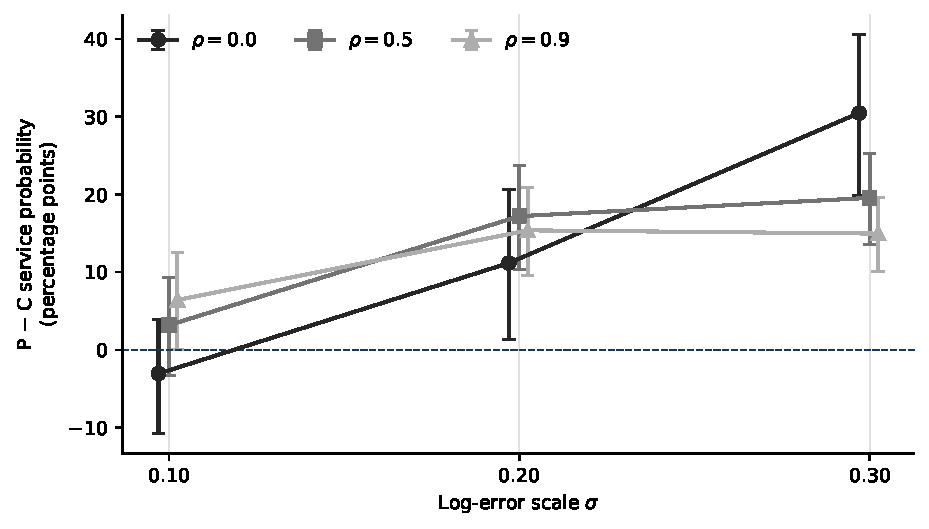
\includegraphics[width=0.93\textwidth]{matched_sensitivity_v7.pdf}
 \caption{Paired original-procedure minus conservative-speed service
 probability on the common 46 instances. Error bars are 95\% bootstrap
 intervals over instances. Plans are fixed across this disturbance sweep;
 the intervals are not simultaneous across cells. Horizontal offsets only
 separate the three correlation series visually.}
 \label{fig:reliability}
\end{figure}

\section{Reproducibility and implementation checks}

The study archive contains the candidate generator, scenario-bank
implementation, test suite, experiment driver, raw JSON records, and the script
that produces the manuscript tables and figure. Tests cover FIFO behavior,
lognormal moments, order-invariant common random numbers, Wilson calculations,
visit and capacity feasibility, and the requirement that contracted candidates
are scored against original windows. Runtime metadata record Python, NumPy,
OR-Tools, operating system, solver budget, seeds, and scenario counts.

The clock convention is essential for reproduction: relative time zero is
06:00 and the evaluator adds 360 minutes before entering the full-day speed
profile. Omitting that offset instead evaluates a 00:00--10:00 shift. The
vectorized evaluator is checked against the original scalar implementation
including period boundaries, customer lateness and shared arc disturbances.

The revision protocol was fixed before running the new candidates. Admission
uses seed $100000+$ instance seed; all fixed outputs are assessed with 5000
fresh scenarios from seed $400000+$ instance seed. The 1000-scenario
disturbance sweep uses seed $500000+$ instance seed. Earlier aggregate results
motivated these analyses, so this is an exploratory extension on known
synthetic instances, not preregistration or an external replication. The
fresh draws do not remove reuse of the instance set. Plans in the sweep are
not re-screened when $\sigma$ or $\rho$ changes. A proposed
confirmatory protocol specifies four directional hypotheses, their tests,
decision rules and failure policy for 53 new instances whose seeds are shifted
by 60000. It becomes fixed when publicly timestamped with a hash manifest of
the code that runs and analyses it. One pipeline smoke test, on an instance
outside that set, was run while the protocol was prepared and is disclosed in
it as pilot data. The protocol's results are not part of this manuscript.

Every reported table and figure is regenerated from retained machine-readable
records. Internal planning buffers are always evaluated against offered
windows, candidate selection and final assessment use independent banks, and
solver-quality comparisons use equal wall-clock budgets and identical
deterministic instances. These rules prevent implementation diagnostics or
adaptive within-run selection from using its own validation outcomes.

\section{Limitations}

First, the generators use nominal or iteratively frozen matrices, so the
procedure can miss better stochastic plans. Conservative speed is uniform
padding, and the clock-aware approximation is not an exact time-dependent
optimizer. Generator and objective choices also differ between screened
families; the experiment is not a full factorial decomposition of every design
decision. Second, the disruption
parameters are assumed, not calibrated to fleet GPS residuals; the results are
conditional on those assumed parameters rather than operational forecasts. An
exploratory $\sigma$--$\rho$ grid is reported, but it does not replace local
calibration. Third,
the geometry is synthetic and the deterministic solver check is not a
substitute for Solomon or Gehring--Homberger benchmarks or a real road network.
Fourth, the AHP weights are one preference vector and require global
sensitivity analysis. Fifth,
Wilson screening addresses binomial sampling uncertainty for a fixed candidate;
its nominal coverage is not a simultaneous guarantee across an adaptively
searched grid. Held-out assessment is therefore necessary. It is also not a
proof of feasibility under distributional misspecification.
Sixth, breakdown recovery, heterogeneous fleets, new-order insertion, and
rolling-horizon replanning are excluded from the present evidence.

\section{Conclusion}

The evidence separates three mechanisms. Uniformly conservative travel times
protect against predictable congestion by construction, padding every trip
including off-peak ones. On matched instances the complete screened procedure
nevertheless exceeds them by \ProcConsRange{} percentage points on average,
although the interval at 200 customers includes zero; for
independent disturbances its advantage grows with noise, from
$\SweepLowIndep$ to \SweepHighIndep{} points. The growth is not monotonic
under strong correlation, so no universal ordering is claimed. The unscreened
slack-aware objective alone does not beat conservative padding; the advantage
belongs to the complete procedure, whose contracted candidate family and
statistical selection act together.

Screening failures are informative rather than opaque. Among the
\FailureCount{} instances without an admitted plan, \CertifiedFailures{}
encounter a certified reachability obstruction at one or more tested
contraction levels. A certificate proves that a particular contracted model is
infeasible; it does not show that reachability alone caused the procedure to
miss its target. Capping each customer's contraction at its
direct-reachability limit raises admission from \OriginalSelected{} to
\CappedSelected{} instances. Of the instances with 100 or 200 customers,
\CappedLargeSelected{} were admitted and \CappedLargeRetained{} retained the
target lower bound under fresh validation, with mean service probability
\CappedLargeRange\%. The gain is not free: it costs \CappedDistanceCost\% more
distance and \CappedFleetCost{} more vehicles on average, rising to
\CappedFleetLarge{} more vehicles at 200 customers. The earlier fleet-matched
experiment concerns the uncontracted objective and does not isolate the
capped variant's mechanism. At 20 customers capping changes nothing; only two
of the six failures there encounter a certificate, and the other four remain
unresolved.

Pooled over all instances, no procedure reaches the 95\% target, so procedure
averages and selected-plan compliance must both be reported. These results are
conditional on assumed disruption parameters and synthetic geometry, and they
are exploratory: the instances that produced them also motivated the design.
The prespecified confirmatory protocol states in advance what fresh
instances must show for the two primary findings to stand.

\section*{Acknowledgments}

The author thanks Thibaut Vidal for guidance on deterministic VRPTW
benchmarking and the use of hybrid genetic search as a comparator, and thanks
the researchers who answered methodological questions by e-mail during the
project. These discussions
informed experimental design; all claims in the paper rest on the reported
model, code, and experiments.

\section*{Data and code availability}

The accompanying reproducibility archive contains source code, dependency
versions, tests, seeds, raw JSON records, analysis scripts, generated tables,
and figures.

\section*{Declarations}

\paragraph{Competing interests.} The author has no relevant financial or non-financial interests to disclose.

\paragraph{Funding.} No external funding supported this study.

\paragraph{Use of generative AI.} Generative AI assistants---OpenAI's
ChatGPT (Astra 6) and Anthropic's Claude (Opus 5, Opus 5.5 and Sonnet 5)---were
used during
this project for code development, experiment implementation, code review,
analysis checking, and drafting and editing text. Every experiment was run from the archived code, every reported number
regenerates from the raw records, and the author takes full responsibility
for the content.

\clearpage
\appendix
\section{AHP pairwise-comparison matrix}\label{sec:ahp-matrix}

Criteria are ordered as distance cost, slack deficit, driver duration and fleet
use. Entry $a_{kl}$ is the judged importance of criterion $k$ relative to $l$
on Saaty's 1--9 scale:
\[
A=\begin{pmatrix}
1 & 3 & 5 & 7\\
1/3 & 1 & 3 & 5\\
1/5 & 1/3 & 1 & 2\\
1/7 & 1/5 & 1/2 & 1
\end{pmatrix}.
\]
Its principal eigenvalue is $\lambda_{\max}=4.0685$, and the normalised
principal eigenvector is
\[
w=(0.5693,\;0.2643,\;0.1055,\;0.0609).
\]
With Saaty's random index 0.90 for four criteria, the consistency index is
$(4.0685-4)/3=0.0228$ and the consistency ratio is $0.0254$. As stated in Section~\ref{sec:objective-scaling},
the third row and column were set when the third criterion was total distance
and were not re-elicited for driver duration.

\section{Additional matched outcomes and failure records}
\begin{table}[H]
\centering
\small
\caption{Customer outcomes on the instances where conservative-speed planning returned a plan. The clock approximation also excludes the instances where it found no schedule, and the counts show this.}
\label{tab:customers}
\begin{tabular}{lrll}
\toprule
Configuration & $k$ & On time (\%) & Expected late\\
\midrule
Nominal & 46 & 83.6 [82.5, 84.6] & 10.00 [7.95, 12.20]\\
Conservative speed & 46 & 93.9 [93.4, 94.4] & 3.47 [2.84, 4.14]\\
Slack-aware & 46 & 90.9 [90.0, 91.7] & 5.46 [4.38, 6.65]\\
Fleet-matched & 46 & 83.0 [81.9, 84.0] & 10.47 [8.29, 12.87]\\
Original procedure & 46 & 96.6 [95.1, 97.9] & 2.20 [1.26, 3.31]\\
Screened conservative & 46 & 97.1 [96.3, 97.8] & 2.20 [1.47, 2.99]\\
Capped procedure & 46 & 97.7 [96.4, 98.9] & 0.91 [0.56, 1.32]\\
Clock approximation & 44 & 88.0 [87.2, 88.7] & 6.73 [5.39, 8.23]\\
\bottomrule
\end{tabular}
\end{table}


\begin{table}[H]
\centering
\scriptsize
\caption{Mean absolute planned resources on the same instances as Table~\ref{tab:customers}: distance in km, scheduled duration in minutes, and vehicles. These are not claims of optimality.}
\label{tab:fullcost}
\begin{tabular}{lrlll}
\toprule
Configuration & $k$ & Distance & Duration & Fleet\\
\midrule
Nominal & 46 & 1180.7 [989.9, 1381.0] & 2906.5 [2379.9, 3481.3] & 7.67 [6.46, 8.98]\\
Conservative speed & 46 & 1216.2 [1021.5, 1422.0] & 3352.5 [2738.5, 4011.0] & 8.30 [6.93, 9.76]\\
Slack-aware & 46 & 1196.3 [1003.0, 1404.0] & 2902.0 [2380.3, 3466.2] & 7.46 [6.22, 8.78]\\
Fleet-matched & 46 & 1174.2 [989.2, 1372.8] & 2833.6 [2330.6, 3382.6] & 7.46 [6.22, 8.76]\\
Original procedure & 46 & 1247.9 [1049.3, 1453.0] & 3171.2 [2620.9, 3777.3] & 8.17 [6.89, 9.57]\\
Screened conservative & 46 & 1252.8 [1056.4, 1461.2] & 3494.5 [2874.0, 4161.0] & 8.76 [7.35, 10.28]\\
Capped procedure & 46 & 1283.5 [1076.5, 1506.8] & 3317.3 [2709.4, 3964.1] & 8.52 [7.13, 10.04]\\
Clock approximation & 44 & 1137.2 [955.5, 1330.9] & 2868.3 [2335.0, 3456.8] & 7.64 [6.32, 9.11]\\
\bottomrule
\end{tabular}
\end{table}


\begin{table}[H]
\centering
\scriptsize
\caption{Sensitivity to the service threshold $\kappa$ on the 46 common instances, with the same plans and the same fresh validation bank in every column. At $n=20/50/100/200$, the number of customers allowed to be late is $2/5/10/20$ at $\kappa=.90$, $1/2/5/10$ at $.95$, $0/1/2/4$ at $.98$, and zero at 1.00.}
\label{tab:kappa}
\begin{tabular}{rlllll}
\toprule
$\kappa$ & N & C & S & P & SC\\
\midrule
0.90 & 38.8 [36.5, 41.2] & 80.6 [78.8, 82.4] & 68.8 [65.9, 71.7] & 89.2 [84.2, 93.7] & 91.2 [88.5, 93.8]\\
0.95 & 21.9 [20.3, 23.5] & 65.6 [63.1, 68.0] & 52.8 [49.9, 55.8] & 83.1 [76.3, 89.4] & 82.8 [77.9, 87.6]\\
0.98 & 11.2 [10.3, 12.2] & 48.2 [45.6, 50.8] & 36.4 [33.8, 39.0] & 75.9 [68.2, 83.3] & 73.2 [67.1, 79.3]\\
1.00 & 6.4 [5.4, 7.4] & 34.4 [31.8, 37.0] & 26.1 [23.8, 28.5] & 68.2 [59.6, 76.2] & 62.4 [53.8, 70.9]\\
\bottomrule
\end{tabular}
\end{table}


\subsection{Instance-level failure audit}\label{sec:failure-audit}

\begin{table}[H]
\centering
\scriptsize
\caption{Every instance on which the original procedure admitted no plan. Best $\beta$ and the lower confidence bound (LCB) refer to the best returned candidate; the no-plan $\beta$ is the first buffer at which the solver returned no plan; the proof $\beta$ is the first buffer with a reachability certificate. Unresolved marks at least one no-plan result without a certificate. A dash means none up to 60 minutes.}
\label{tab:failure}
\begin{tabular}{rrrrrrc}
\toprule
$n$ & Seed & Best $\beta$ & LCB (\%) & No-plan $\beta$ & Proof $\beta$ & Unresolved\\
\midrule
20 & 7200 & 45 & 90.7 & 50 & -- & Yes\\
20 & 7201 & 35 & 93.5 & 40 & -- & Yes\\
20 & 7210 & 35 & 90.8 & 45 & -- & Yes\\
20 & 7212 & 5 & 37.9 & 10 & -- & Yes\\
20 & 7216 & 55 & 90.7 & 60 & 60 & No\\
20 & 7218 & 10 & 65.9 & 15 & 50 & Yes\\
50 & 7501 & 25 & 87.5 & 30 & 35 & Yes\\
50 & 7503 & 10 & 64.1 & 15 & 15 & No\\
50 & 7504 & 35 & 91.3 & 40 & 40 & No\\
50 & 7506 & 0 & 44.7 & 5 & 5 & No\\
50 & 7508 & 35 & 85.9 & 40 & 40 & No\\
50 & 7511 & 35 & 88.5 & 40 & 50 & Yes\\
50 & 7513 & 40 & 93.6 & 45 & 60 & Yes\\
100 & 8003 & 20 & 85.3 & 25 & 25 & No\\
100 & 8004 & 15 & 81.5 & 20 & 20 & No\\
100 & 8007 & 5 & 73.6 & 15 & 15 & No\\
100 & 8008 & 25 & 91.7 & 35 & 35 & No\\
200 & 9004 & 10 & 71.2 & 15 & 15 & No\\
200 & 9005 & 20 & 88.9 & 25 & 25 & No\\
200 & 9006 & 25 & 94.9 & 40 & 40 & No\\
200 & 9007 & 20 & 86.4 & 25 & 25 & No\\
\bottomrule
\end{tabular}
\end{table}


\begin{table}[H]
\centering
\small
\caption{Retained equal-budget benchmark on the deterministic core: excess distance of OR-Tools routes over PyVRP/HGS routes (\%). Counts are valid pairs at the one-second and five-second budgets; one pair is missing at one second.}
\label{tab:hgs}
\begin{tabular}{rrll}
\toprule
$n$ & Valid pairs (1s/5s) & One second & Five seconds\\
\midrule
20 & 19/20 & 1.0 [0.3, 1.8] & 0.0 [0.0, 0.0]\\
50 & 15/15 & 4.8 [3.3, 6.2] & 3.0 [1.9, 4.2]\\
100 & 10/10 & 8.5 [5.9, 11.1] & 6.3 [4.7, 7.9]\\
200 & 8/8 & 32.9 [29.4, 36.2] & 11.1 [9.3, 13.5]\\
\bottomrule
\end{tabular}
\end{table}

\clearpage

\begingroup
\small
\begin{thebibliography}{99}

\bibitem{ahmed2008}
Ahmed, S., and Shapiro, A. (2008). Solving chance-constrained stochastic
programs via sampling and integer programming. In Z.-L. Chen and S. Raghavan
(eds.), \emph{State-of-the-Art Decision-Making Tools in the
Information-Intensive Age}, TutORials in Operations Research, 261--269.
INFORMS, Hanover, MD. DOI: 10.1287/educ.1080.0048.

\bibitem{bomboi2022}
Bomboi, F., Buchheim, C., and Pruente, J. (2022). On the stochastic vehicle
routing problem with time windows, correlated travel times, and time
dependency. \emph{4OR}, 20(2), 217--239. DOI:
10.1007/s10288-021-00476-z.

\bibitem{brown2001}
Brown, L. D., Cai, T. T., and DasGupta, A. (2001). Interval estimation for a
binomial proportion. \emph{Statistical Science}, 16(2), 101--133. DOI:
10.1214/ss/1009213286.

\bibitem{ehmke2015}
Ehmke, J. F., Campbell, A. M., and Urban, T. L. (2015). Ensuring service
levels in routing problems with time windows and stochastic travel times.
\emph{European Journal of Operational Research}, 240(2), 539--550. DOI:
10.1016/j.ejor.2014.06.045.

\bibitem{errico2018}
Errico, F., Desaulniers, G., Gendreau, M., Rei, W., and Rousseau, L.-M. (2018).
The vehicle routing problem with hard time windows and stochastic service
times. \emph{EURO Journal on Transportation and Logistics}, 7(3), 223--251.
DOI: 10.1007/s13676-016-0101-4.

\bibitem{ghiani2014}
Ghiani, G., and Guerriero, E. (2014). A note on the Ichoua, Gendreau, and
Potvin travel time model. \emph{Transportation Science}, 48(3), 458--462.
DOI: 10.1287/trsc.2013.0491.

\bibitem{ichoua2003}
Ichoua, S., Gendreau, M., and Potvin, J.-Y. (2003). Vehicle dispatching with
time-dependent travel times. \emph{European Journal of Operational Research},
144(2), 379--396. DOI: 10.1016/S0377-2217(02)00147-9.

\bibitem{li2010}
Li, X., Tian, P., and Leung, S. C. H. (2010). Vehicle routing problems with
time windows and stochastic travel and service times: Models and algorithm.
\emph{International Journal of Production Economics}, 125(1), 137--145.
DOI: 10.1016/j.ijpe.2010.01.013.

\bibitem{ortools}
Perron, L., and Furnon, V. (2026). OR-Tools. Google.
\url{https://developers.google.com/optimization}

\bibitem{saaty1980}
Saaty, T. L. (1980). \emph{The Analytic Hierarchy Process}. McGraw-Hill.

\bibitem{serrano2026}
Serrano, B., Florio, A. M., Minner, S., Schiffer, M., and Vidal, T. (2026).
Contextual stochastic vehicle routing with time windows.
\emph{INFORMS Journal on Computing}. DOI: 10.1287/ijoc.2025.1189.

\bibitem{solomon1987}
Solomon, M. M. (1987). Algorithms for the vehicle routing and scheduling
problems with time window constraints. \emph{Operations Research}, 35(2),
254--265. DOI: 10.1287/opre.35.2.254.

\bibitem{tas2014}
Ta\c{s}, D., Dellaert, N., van Woensel, T., and de Kok, A. G. (2014). The
time-dependent vehicle routing problem with soft time windows and stochastic
travel times. \emph{Transportation Research Part C}, 48, 66--83. DOI:
10.1016/j.trc.2014.08.007.

\bibitem{toth2014}
Toth, P., and Vigo, D. (eds.) (2014). \emph{Vehicle Routing: Problems, Methods,
and Applications}, 2nd ed. SIAM. DOI: 10.1137/1.9781611973594.

\bibitem{vareias2019}
Vareias, A. D., Repoussis, P. P., and Tarantilis, C. D. (2019). Assessing
customer service reliability in route planning with self-imposed time windows
and stochastic travel times. \emph{Transportation Science}, 53(1), 256--281.
DOI: 10.1287/trsc.2017.0748.

\bibitem{wilson1927}
Wilson, E. B. (1927). Probable inference, the law of succession, and
statistical inference. \emph{Journal of the American Statistical Association},
22(158), 209--212. DOI: 10.1080/01621459.1927.10502953.

\bibitem{wouda2024}
Wouda, N. A., Lan, L., and Kool, W. (2024). PyVRP: A high-performance VRP
solver package. \emph{INFORMS Journal on Computing}, 36(4), 943--955. DOI:
10.1287/ijoc.2023.0055.

\end{thebibliography}
\endgroup

\end{document}
